\documentclass[12pt]{article}
\usepackage{inputenc}
\usepackage[russian]{babel}
\title{Решение задачи построения максимальной зелёной волны графоаналитическим способом}
\author{Красник А.Л.}
\date{Москва 2025.}
\usepackage{graphics}
\usepackage{graphicx}
\DeclareGraphicsExtensions{.pdf, .jpeg,.jpg,.png,.tif}
\usepackage{fontenc}
\usepackage{placeins}
\usepackage{booktabs}
\usepackage{graphicx}

\begin{document}
\maketitle
\newpage
\section{Задача}
Реализовать алгоритм графоаналитического метода нахождения максимальной "зелёной волны" и с его помощью решить задачу с конкретными данными. Найти такие смещения (сдвиги) светофорных лент, чтобы обеспечить максимальное количество и максимальную ширину "зелёных волн". Допускается изменять длительность сигналов светофоров в заданных диапазонах.
\section{Данные светофорных объектов}
\begin{table}[h!]
\centering
\caption{Координаты светофорных объектов и расстояния между ними}
\begin{tabular}{cccccc}
\toprule
Светофорный объект & Имя & X & Y & Дистанция до следующего (м) \\
\midrule
0 & tls \#0 & 0   & 0   & 200 \\
1 & tls \#1 & 0   & 200 & 250 \\
2 & tls \#2 & 0   & 450 & 150 \\
3 & tls \#3 & 0   & 600 & --  \\
\bottomrule
\end{tabular}
\end{table}

\begin{table}[h!]
\centering
\small
\caption{Фазы и сигналы для светофорных объектов. Сигналы в каждой фазе идут последовательно. Суммарная длительность фазы (т.е. \textit{цикл}) — 85 секунд}
\begin{tabular}{|p{2.6cm}|p{3.2cm}|p{1.4cm}|p{3.2cm}|p{1.5cm}|p{1.5cm}|}
\hline
\textbf{Светофорный объект} & \textbf{Идентификатор фазы} & \textbf{Сигнал} & \textbf{Длительность сигнала (с)} & \textbf{Мин. дл-ть (с)} & \textbf{Макс. дл-ть (с)} \\
\hline
0 & 1 & Green & 30 & 25 & 35 \\
0 & 1 & Red   & 20 & 20 & 20 \\
0 & 2 & Green & 20 & 15 & 25 \\
0 & 2 & Red   & 15 & 15 & 15 \\
\hline
1 & 10 & Red   & 20 & 20 & 20 \\
1 & 10 & Green & 35 & 30 & 40 \\
1 & 10 & Yellow& 5  & 5  & 5  \\
1 & 11 & Red   & 10 & 10 & 10 \\
1 & 11 & Green & 10 & 5  & 15 \\
1 & 11 & Yellow& 5  & 5  & 5  \\
\hline
2 & 20 & Red   & 45 & 45 & 45 \\
2 & 20 & Green & 10 & 5  & 15 \\
2 & 21 & Red   & 7  & 7  & 7  \\
2 & 21 & Green & 18 & 18 & 18 \\
2 & 21 & Yellow& 5  & 5  & 5  \\
\hline
3 & 30 & Red   & 40 & 40 & 40 \\
3 & 30 & Green & 15 & 10 & 20 \\
3 & 31 & Red & 10 & 10 & 10 \\
3 & 31 & Green & 20 & 20 & 20 \\
\hline
\end{tabular}
\end{table}

\newpage

\section{Блок-схема}
\begin{figure}[h!]
  \centering
  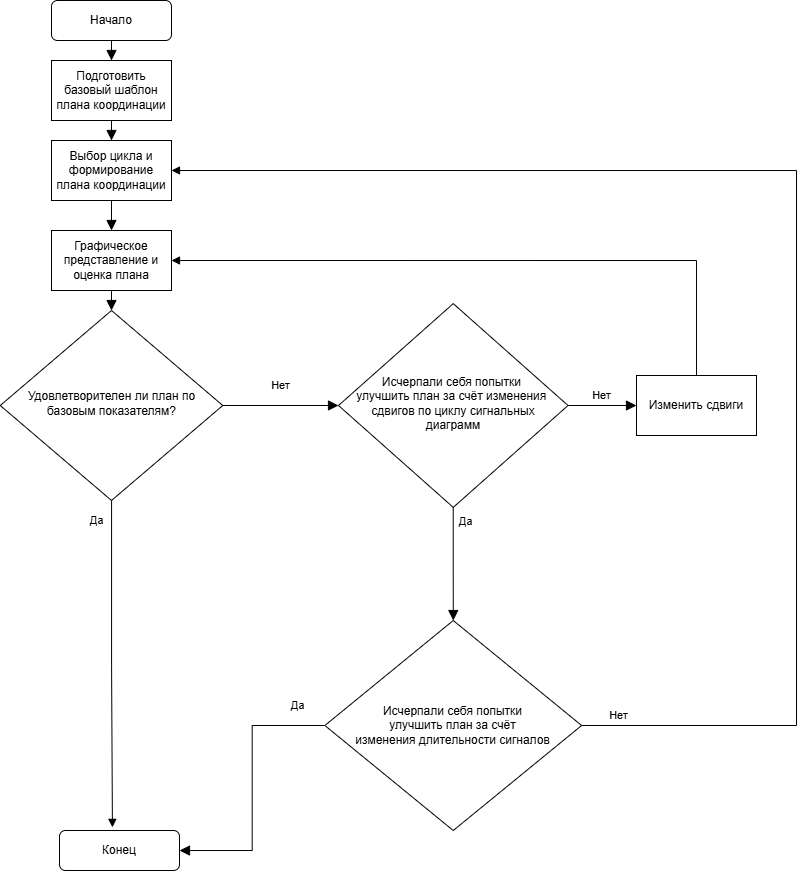
\includegraphics[width=1.1\textwidth]{Block_diagram.png} 
  \caption{Блок-схема графоаналитического метода} 
  \label{fig:diagram} 
\end{figure}
\end{document}